A paper equilateral triangle $ABC$ has side length $12$. The paper triangle is folded so that vertex $A$ touches a point on side $\overline{BC}$ a distance $9$ from point $B$. The length of the line segment along which the triangle is folded can be written as $\frac{m\sqrt{p}}{n}$, where $m$, $n$, and $p$ are positive integers, $m$ and $n$ are relatively prime, and $p$ is not divisible by the square of any prime. Find $m+n+p$.
\begin{center}
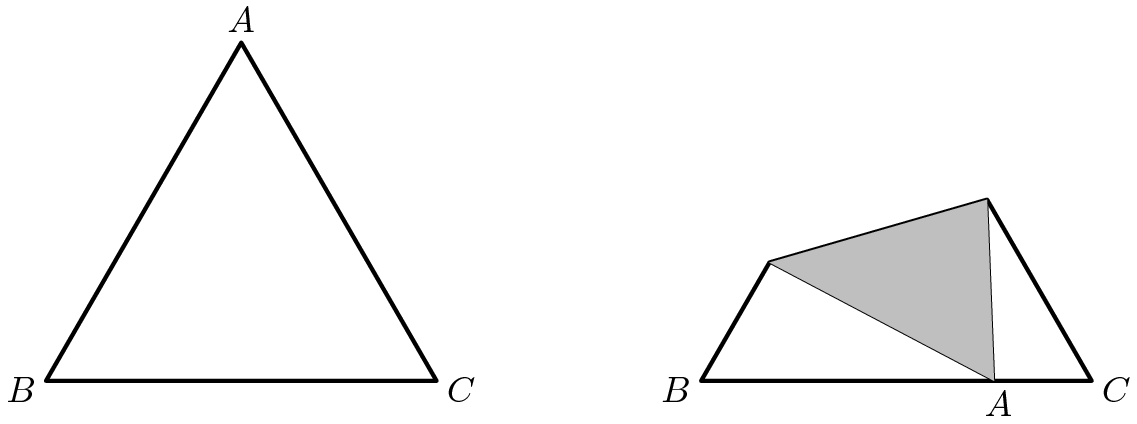
\includegraphics[width = 113.60000000000001mm]{img/fig0.png}
\end{center}